\documentclass[12pt, a4paper]{article}
\usepackage{fullpage}
\usepackage{amsmath}
\usepackage{graphicx}
\usepackage{natbib}
\usepackage{tikz}
\usepackage{tikz-dimline} \pgfplotsset{compat=newest}
\title{Open Channel Flow with Manning's Equation}
\author{Guoping Tang}
\date\today{}

\begin{document}
\maketitle

\begin{abstract}
Equations for analytical and numerical solutions involving Manning's equation are derived for triangular, rectangular, trapezoidal, and parabolic open channels and circular, elliptical, and arch closed conduits.
\end{abstract}

\section{Theory}
\subsection{Manning's Equation}
The Manning's equation for the velocity and discharge of uniform flow in open channels is \cite{Chow1959,French1985,Munson2013,hds4}:
\begin{equation}  
v = \frac{K_u}{n}R^{\frac{2}{3}}S^{\frac{1}{2}},
\label{Eq:v}
\end{equation}
\begin{equation}  
Q = vA = \frac{K_u}{n}AR^{\frac{2}{3}}S^{\frac{1}{2}}=\frac{K_u}{n}A^{\frac{5}{3}}P^{-\frac{2}{3}}S^{\frac{1}{2}},
\label{Eq:Q}
\end{equation}
where
\begin{itemize}
\item[] $v$ = Mean velocity, m/s (ft/s),
\item[] $Q$ = Discharge, $m^3/s$ ($ft^3/s$),
\item[] $n$ = Manning's coefficient of roughness,
\item[] $R$ = Hydraulic radius, m (ft). $R = P/A$,
\item [] $P$ = Wetted perimeter, m (ft),
\item [] $A$ = Crossing-section area of flowing water perpendicular to the direction of flow, $m^2$ ($ft^2$),
\item[] $S$ = Energy slope, m/m (ft/ft). For steady uniform flow $S=S_0$ , and
\item[] $K_u$ = units conversion factor, 1 for SI, 1.486 for English units.
\end{itemize}

\subsection{Normal Depth}
Depending on the geometry of the channel, both $A$ and $P$ are depdent on normal depth $y$. To calculate $y$ for a given $Q$, we solve 

\begin{equation}  
f_d(y_{i})= \frac{K_u}{n}A^{\frac{5}{3}}P^{-\frac{2}{3}}S^{\frac{1}{2}} - Q 
\end{equation}

\noindent for $f_d(y_{i}) = 0$. Analytical solutions are available in some special cases, for example, triangular channels. In general, a numerical solution is used to solve the nonlinear equation iteratively. Using Newton's method \cite{Strang1991}, the iteration starts with an initial guess $y_0$, and iterates with
\begin{equation}  
y_{i+1} = y_i -\frac{f_d(y_{i})}{f_d'(y_{i})}
\end{equation}
where
\begin{equation}  
f'_d(y_{i})=\frac{\partial f_d}{\partial y}= \frac{K_u}{n}S^{\frac{1}{2}}\left(\frac{5}{3}R^{\frac{2}{3}}\frac{\partial A}{\partial y} -  \frac{2}{3}R^{\frac{5}{3}}\frac{\partial P}{\partial y}\right)
\end{equation}

\noindent until 
\begin{equation}  
|f_d(y_{i})| \leq TOLQ, 
\label{Eq:TOLQ}
\end{equation}

\begin{equation}  
|y_{i+1} - y_i| \leq TOLD, 
\label{Eq:TOLD}
\end{equation}

\noindent or 
\begin{equation}  
i \geq MAXI 
\label{Eq:MAXI}
\end{equation}
with 
\begin{itemize}
\item[] $TOLQ$ = discharge tolerance, $m^3/s$ ($ft^3/s$),
\item[] $TOLD$ =depth tolerance, $m$ ($ft$),
\item[] $MAXI$ = maximum number of iteration.
\end{itemize}

\noindent When the iteration stops with criteria Eq.(\ref{Eq:MAXI}), an error is shown to notify the user. The user may adjust $y_0$ or $t_0$, $TOLQ$, $TOLD$, and/or $MAXI$ to obtain a satisfactory solution. 

\noindent For circular, elliptical, and arch pipes, a replacement of variable $y$ with an alternative variable $t$ (for example) is convient. These equations remain valid. An alternative tolerance $TOLA$ (in lieu of $TOLD$) is specified when $t$ is an angle.

For open channel flow in closed conduits such as circular, elliptical, and arch pipes, the calculated discharge peaks before the pipe is full \cite{Chow1959,French1985,Munson2013}. 
The normal depth $y_{max}$ or $t_{max}$ at peak discharge $Q_{max}$ can be calculated by solving
\begin{equation}  
\frac{\partial Q}{\partial t} = \frac{K_u}{n} \left(\frac{5}{3}R^{\frac{2}{3}}\frac{\partial A}{\partial t} -  \frac{2}{3}R^{\frac{5}{3}}\frac{\partial P}{\partial t}\right) S^{\frac{1}{2}}=0.
\end{equation}
or
\begin{equation}  
f(t) = 5P\frac{\partial A}{\partial t} -  2 A\frac{\partial P}{\partial t} = 5PA' -  2 AP' = 0.
\label{Eq:MaxQ}
\end{equation}

\noindent In absence of an analytical solution, Newton's method is used with
\begin{equation}  
t _{i+1} = t _i - \frac{f(t _i)}{f'(t_i)},
\end{equation}
\begin{equation}  
f'(t_i) = 5A''P  + 3A'P' - 2AP''.
\end{equation}

\noindent If $Q > Q_{max}$ , an error is shown with $y_{max}$ returned as normal depth.  

\noindent In cases where $Q$ is not a monotonically increasing function with $y$, multiple $y$ values may result in the same $Q$ value. The lowest value is returned as normal depth. 

\noindent In summary, to calculate normal depth with Newton's method, we need A, P, A' and  P'. A'' and P'' are needed when $Q_{max}$ needs to be calculated using Newton's method.

\subsection{Critical Depth}
Critical flow occurs when the specific energy
\begin{equation}
E = \frac{v^2}{2g} + y =\frac{Q^2}{2gA^2} + y 
\end{equation}
reaches a minimum ($g$ is acceleration of gravity, 32.17 $ft/s^2$ for US Customery units, 9.81 $m/s^2$ for SI). Namely,
\begin{equation}
\frac{\partial E}{\partial y} =  -\frac{Q^2}{gA^3}\frac{\partial A}{\partial y} + 1 = 0.
\end{equation}
To solve the equation with Newton's method, critical depth $y_c$ or $t_c$ is calculated by
\begin{equation}  
t_{c,i+1} = t_{c,i} -\frac{f(t_{c,i})}{f'(t_{c,i})}
\end{equation}
where
\begin{equation}  
f_c(t)= gA^3 - Q^2\frac{\partial A}{\partial y} 
\label{Eq:C}
\end{equation}

\begin{equation}  
f'_c(t)= 3gA^2\frac{\partial A}{\partial t} - Q^2\frac{\partial}{\partial t}\left(\frac{\partial A}{\partial y}\right) 
\end{equation}

\noindent The critical velocity $v_c$ is 
\begin{equation}
v_c = \frac{Q}{A_c} = \sqrt{g \frac{A}{\frac{\partial A}{\partial y}}} = \sqrt{gD}
\end{equation}
where $D = A/\frac{\partial A}{\partial y}$ is the hydraulic depth.

\noindent The Froude number, $F = v/v_c$. The critical slope $S_c$ is backcalculated from Eq. (\ref{Eq:v}).

%\begin{equation}  
%f_c(y_{i})= 1 - \frac{Q^2}{gA^3}\frac{\partial A}{\partial y} 
%\end{equation}

%\begin{equation}  
%f'_c(y_{i})= \frac{Q^2}{gA^3} \left[ 3 \left(\frac{\partial A}{\partial y}\right)^2 - A\frac{\partial ^2 A}{\partial y^2}   \right] 
%\end{equation}

%for A and y are parameterized as a function of $t$ with $A=A(t)$, $A'=\frac{\partial A(t)} {\partial t}$, $y=y(t)$, $y'=\frac{\partial y(t)}{\partial t}$, 

%For $y=y_c$,
%\begin{equation}
%Q_c^2 = \frac{gA^3}{\frac{\partial A}{\partial y}} 
%\end{equation}

%\begin{equation}  
%t_{c,i+1} = t_{c,i} -\frac{f(t_{c,i})}{f'(t_{c,i})}
%\end{equation}

%\begin{equation}  
%f_c(t)= gA^3(t) - Q^2\frac{\partial A}{\partial y}(t) = gA^3 - Q^2 A' / y'
%\end{equation}

%\begin{equation}  
%f'_c(t)= 3gA^2\frac{\partial A}{\partial t} - Q^2\frac{\partial}{\partial t}\left(\frac{\partial A}{\partial y}\right) = 3gA^2A' - Q^2 \frac{A''y' - A'y''}{y'^2}
%\end{equation}

%\begin{equation}  
%f_c(t)= 1 - \frac{Q^2}{gA^3}\frac{A'}{y'} 
%\end{equation}

%\begin{equation}  
%f'_c(t)= \frac{Q^2}{gA^3} \left[ 3 \left(\frac{\partial A}{\partial y}\right)^2 - A\frac{\partial ^2 A}{\partial y^2}   \right] 
%\end{equation}



\section{Triangular}

\begin{figure}[h]
\centering
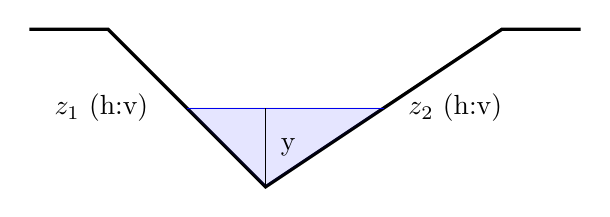
\begin{tikzpicture}
\draw[very thick] (0,0) -- (1,0) -- node[left=10pt]{$z_1$ (h:v)}(3,-2)--node[right=5]{$z_2$ (h:v)} (6,0) -- (7,0);
\draw[blue] (2,-1) -- (4.5,-1);

\filldraw[fill=blue, opacity=0.1](2, -1) --(4.5, -1) -- (3, -2);


\draw (3,-2)--node[right=2]{y} (3,-1);
\end{tikzpicture}
\caption{Triangular Section}
\end{figure}

\begin{equation}
A = \frac{1}{2} (z_1 + z_2) y^2
\end{equation}

\begin{equation}
P = \left(\sqrt{1+z_1^2} + \sqrt{1+z_2^2}\right)y
\end{equation}

\begin{equation}
R = \frac{1}{2}\frac{(z_1 + z_2) }{\sqrt{1+z_1^2} + \sqrt{1+z_2^2}}y
\end{equation}
For normal flow, Eq. (\ref{Eq:Q}) becomes
\begin{equation}
Q = \frac{K_u}{n} \frac{z_1 + z_2}{2}  \left(\frac{1}{2}\frac{z_1 + z_2}{\sqrt{1+z_1^2} + \sqrt{1+z_2^2}}\right)^{\frac{2}{3}} y^{\frac{8}{3}}S^{\frac{1}{2}}.
\end{equation}
Note this equation can be used to backcalculate normal depth $y_n$ from $Q$.
\begin{equation}
\frac{\partial A}{\partial y} = (z_1 + z_2)y = T_w
\end{equation}
with $T_w$ as the width of the water surface.

\noindent For critical flow, Eq. (\ref{Eq:C}) becomes
\begin{equation}  
f_c(y)= \frac{g}{8}(z_1 + z_2)^3y^6 - Q^2(z_1 + z_2)y = 0.
\end{equation}

\begin{equation}  
y_c^5 = \frac{8Q^2}{g(z_1 + z_2)^2}
\end{equation}

\begin{equation}  
D_h = \frac{A}{\frac{\partial A}{\partial y}} = \frac{\frac{1}{2} (z_1 + z_2) y^2}{(z_1 + z_2)y} = \frac{1}{2}(z_1 + z_2)y_c
\end{equation}

\begin{equation}  
v_c = \sqrt{\frac{1}{2}g(z_1 + z_2)y_c}
\end{equation}


\section{Rectangular}

\begin{figure}[h]
\centering
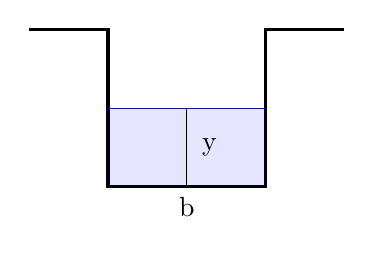
\begin{tikzpicture}
\draw[very thick] (0,0) -- (1,0) -- (1,-2)--node[below]{b}(3, -2) -- (3,0) -- (4,0);
\draw[blue] (1,-1) -- (3,-1);
\filldraw[fill=blue, opacity=0.1](1, -1) --(3, -1) -- (3, -2) -- (1,-2);
\draw (2,-2)--node[right=2]{y} (2,-1);
\end{tikzpicture}
\caption{Rectangular Section}
\end{figure}

\begin{equation}
A = by
\end{equation}

\begin{equation}
P = b + 2y
\end{equation}

\begin{equation}
R = \frac{by}{b+2y}
\end{equation}

\begin{equation}
\frac{\partial A}{\partial y} = b = T_w
\end{equation}

\begin{equation}  
f_c(y)= gb^3y^3 -Q^2b= 0
\end{equation}

\begin{equation}  
y_c^3 = \frac{Q^2}{gb^2}
\end{equation}

\begin{equation}  
D_h = \frac{A}{\frac{\partial A}{\partial y}} = \frac{by_c}{b} = y_c
\end{equation}

\begin{equation}  
v_c = \sqrt{g y_c}
\end{equation}

\noindent Neton's method is used to calculate normal depth $y_n$.
\section{Trapezoidal}
\begin{figure}[h]
\centering
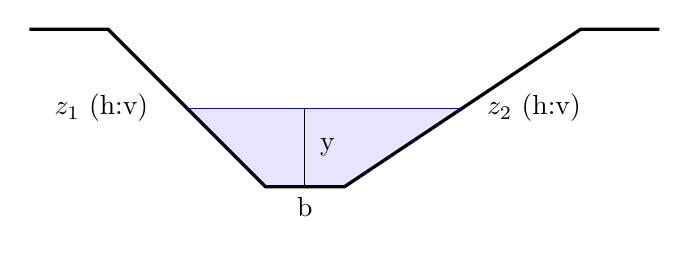
\begin{tikzpicture}
\draw[very thick] (0,0) -- (1,0) -- node[left=10pt]{$z_1$ (h:v)}(3,-2)--node[below]{b}(4,-2)--node[right=5]{$z_2$ (h:v)} (7,0) -- (8,0);
\draw[blue] (2,-1) -- (5.5,-1);
\filldraw[fill=blue, opacity=0.1](2, -1) --(5.5, -1) -- (4, -2) -- (3, -2);

\draw (3.5,-2)--node[right=2]{y} (3.5,-1);
\end{tikzpicture}
\caption{Trapezoidal Section}
\end{figure}

\begin{equation}
A = \frac{1}{2} (z_1 + z_2) y^2 + by
\end{equation}

\begin{equation}
P = \left(\sqrt{1+z_1^2} + \sqrt{1+z_2^2}\right)y + b
\end{equation}

\begin{equation}
\frac{\partial A}{\partial y} = (z_1 + z_2)y + b
\end{equation}

\begin{equation}
\frac{\partial ^2A}{\partial y^2} = z_1 + z_2
\end{equation}

\begin{equation}
\frac{dP}{dy} = \sqrt{1+z_1^2} + \sqrt{1+z_2^2}
\end{equation}


\section{Parabolic}

\begin{figure}[h]
\centering
\begin{tikzpicture}
\draw[very thick] (0,0) parabola (2, 3);
\draw[very thick] (0,0) parabola (-2, 3);
%\dimline [extension start length=0.1, extension end length=0.1]{(-2, 3.5)}{(2, 3.5)}{T}
\dimline [extension start length=0.1, extension end length=0.1]{(2.5,3)}{(2.5, 0)}{d}
\dimline [extension start length=0.1, extension end length=0.1]{(0,-3.5)}{(2, -3.5)}{T/2}
\draw[blue] (-1, 0.75) -- (1, 0.75);
%\filldraw[fill=blue, opacity=0.1](-2.828, -4.242) arc[x radius=4, y radius = 6, start angle = 225, end angle=315];
\draw (0,0)--node[right=3]{y} (0,1.6875);

\draw (2, 3) -- (0, -3);

\draw[->](-4,0) --(4, 0) node[below =6]{x} ;
\draw[->](0, -4) --(0,4);


\end{tikzpicture}
\end{figure}

\noindent For a parabola with top width $T$ and depth $d$,
\begin{equation}  
y= 4\frac{d}{T^2}x^2
\end{equation}
 
\begin{equation}  
A= 2xy - \int_{-x}^x 4\frac{d}{T^2}x^2 dx = \frac{16}{3}\frac{d}{T^2}x^3 = \frac{2}{3}\frac{T}{\sqrt{d}}y^{\frac{3}{2}}
\end{equation}

\begin{equation}  
\frac{\partial A}{\partial y}= T\sqrt{\frac{y}{d}} = 2x = T_w
\end{equation}

\begin{equation}  
\frac{\partial ^2A}{\partial y^2}= \frac{T}{2\sqrt{yd}}
\end{equation}

\noindent To calculate $P$ % and $P'$,
\begin{equation}  
\frac{\partial y}{\partial x}= 8\frac{d}{T^2}x
\end{equation}

\begin{equation}  
\left(\frac{\partial y}{\partial x}\right)^2 = 8\frac{d}{T^2}8\frac{d}{T^2} x^2 = 16\frac{d}{T^2}y =  \frac{y}{a}
\end{equation}
with $a = T^2/16d$

\begin{equation}  
\frac{\partial P}{\partial y}= 2\sqrt{1 + (dx/dy)^2} = 2\sqrt{1 + \frac{a}{y}}
\end{equation}



%\begin{equation}  
%\int \sqrt{1+\frac{a}{t}}dt = \frac{a}{2}\ln\left(\sqrt{1+\frac{a}{t}} +1\right) 
%                                              - \frac{a}{2}\ln\left(|\sqrt{1+\frac{a}{t}} -1|\right)
%                                             + x\sqrt{1+\frac{a}{t}} + c 
%%\end{equation}
\begin{equation}  
\int \sqrt{1+\frac{a}{t}}dx = \frac{a}{2}\ln \frac{\sqrt{1+\frac{a}{t}} +1}{\sqrt{1+\frac{a}{t}} -1} 
                                             + \sqrt{t^2+at} + c 
                                             = \frac{a}{2}\ln \frac{\sqrt{t^2+at} +t}{\sqrt{t^2+at} -t} 
                                             + \sqrt{t^2+at} + c 
\end{equation}

\noindent Let $b = \sqrt{y^2 + ay}$,
\begin{equation}  
P= 2\int_0^y \sqrt{1 + \frac{a}{y}}dy = = a \ln \frac{b + y}{b -  y} + 2b
\end{equation}

\begin{equation}  
D_h = \frac{A}{\frac{\partial A}{\partial y}} = \frac{ \frac{2}{3}\frac{T}{\sqrt{d}}y^{\frac{3}{2}}}{T\sqrt{\frac{y}{d}}} = \frac{2}{3}y_c
\end{equation}

\begin{equation}  
v_c = \sqrt{\frac{2}{3}gy_c}
\end{equation}

\noindent Neton's method is used to calculate normal depth $y_n$ and critical depth $y_c$. An initial guess for critical depth \cite{French1985} is
\begin{equation}
y_{c,0} =  \left(0.84 \frac{4dQ^2}{gT}\right)^{0.25}
\end{equation}


\section{Irregular}
\begin{figure}[h]
\centering
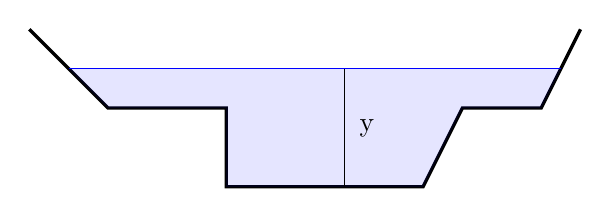
\begin{tikzpicture}
\draw[very thick] (0,0) -- (1,-1) -- (2.5,-1)--(2.5, -2) --(5, -2)-- (5.5, -1) -- (6.5,-1) --(7,0);
\draw[blue] (0.5,-0.5) -- (6.75,-0.5);
\filldraw[fill=blue, opacity=0.1](0.5, -0.5) -- (1,-1) -- (2.5,-1)--(2.5, -2) --(5, -2)-- (5.5, -1) -- (6.5, -1) -- (6.75, -0.5);
\draw (4,-2)--node[right=2]{y} (4,-0.5);
\end{tikzpicture}
\caption{Irregular Section}
\end{figure}

\subsection{Composite Roughness}

\noindent Pavlovskii's method

\noindent Assumption: the total force-resisting motion is equal to the sum of the subsection-resisting forces.

\begin{equation}
nP^2 = \sum n_iP_i^2
\end{equation}

\noindent Horton's method

\noindent Assumption: each subdivision has the same average velocity of the total section
\begin{equation}
Pn^{3/2} = \sum P_i  n_i^{3/2}
\end{equation}

\noindent Colebatch method

\begin{equation}
An^{3/2} = \sum A_i  n_i^{3/2}
\end{equation}

\noindent Cox method

\begin{equation}
An = \sum A_i  n_i
\end{equation}

\noindent Lotter method

\noindent Assumption: the total discharge is eqal to the sum of the subsection discharges.

\begin{equation}
\frac{PR^{5/3}}{n} = \sum \frac{P_i  R_i^{5/3}}{n_i}
\end{equation}

\section{Circular}

\begin{figure}[h]
\centering
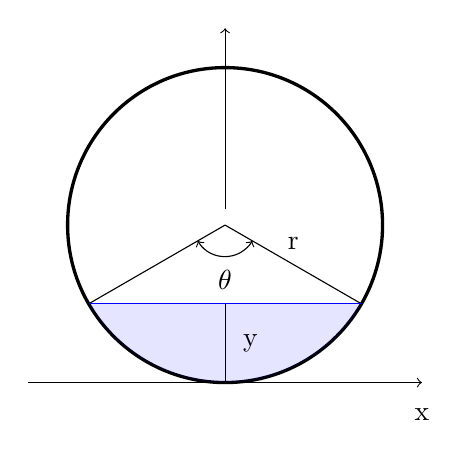
\begin{tikzpicture}
\draw[very thick] (0,0) circle (2);
\draw (0,0)--node[above=2]{r} (1.732051, -1);
\draw (0,0)--(-1.732051, -1);

\draw [<->] (-0.3464, -0.2) arc [radius=0.4, start angle=210, end angle=330];

\node at (0, -0.7) {$\theta$};

\draw[blue] (-1.732051, -1) -- (1.732051, -1);

\filldraw[fill=blue, opacity=0.1](-1.732, -1) arc[x radius=2, y radius = 2, start angle = 210, end angle=330];

\draw (0,-1)--node[right=3]{y} (0,-2);

\draw[->](-2.5,-2) --(2.5, -2) node[below =6]{x} ;
\draw[->](0, 0.2) --(0,2.5);

\end{tikzpicture}
\caption{Circular Section}
\end{figure}

%\subsection{Basic Equations}
\begin{equation}
y = r(1 - \cos\frac{\theta}{2})
\end{equation}

\begin{equation}
A = \frac{1}{2} (\theta - \sin\theta) r^2
\end{equation}

\begin{equation}
P =  \theta r
\end{equation}

\begin{equation}
R = \frac{1}{2} \left(1 - \frac{\sin\theta}{\theta} \right) r
\end{equation}

%\begin{equation}
%T_w = 2r \sin \frac{\theta}{2}
%\end{equation}

\begin{equation}
\frac{\partial y}{\partial \theta} = \frac{r}{2}\sin \frac{\theta}{2}
\end{equation}

\begin{equation}
\frac{\partial A}{\partial \theta} = \frac{1}{2} (1 - \cos\theta) r^2
\end{equation}

\begin{equation}
\frac{\partial A}{\partial y} = \frac{\frac{\partial A}{\partial \theta}}{\frac{\partial y}{\partial \theta}} = \frac{\frac{1}{2} (1 - \cos\theta) r^2}{\frac{r}{2}\sin \frac{\theta}{2}} = 2r\sin\frac{\theta}{2}
\end{equation}

\begin{equation}
\frac{\partial}{\partial \theta}\left(\frac{dA}{dy}\right) = r\cos\frac{\theta}{2} = T_w
\end{equation}

\begin{equation}
\frac{\partial P}{\partial \theta} =  r
\end{equation}

%\begin{equation}
%\frac{dT}{d\theta} = r \cos \frac{\theta}{2}
%\end{equation}

%\subsection{Calculate Maximum Discharge Using Manning's Equation}
%\begin{equation}  
%Q = \frac{K_u}{n}AR^{2/3}S^{1/2} = \frac{K_u}{n}A^{5/3}P^{-2/3}S^{1/2},
%\end{equation}

%\begin{equation}  
%\frac{dQ}{d\theta} = \frac{K_u}{n} \left(\frac{5}{3}R^{2/3}\frac{\partial A}{\partial \theta} -  \frac{2}{3}R^{5/3}\frac{\partial P}{\partial \theta} \right) S^{1/2}=0,
%\end{equation}
%
%\begin{equation}  
%5\frac{\partial A}{\partial \theta} -  2 R\frac{\partial P}{\partial \theta} = 0,
%\label{Eq:CircularMaxQ}
%\end{equation}

\noindent To calculate $\theta_{max}$, $y_{max}$, and $Q_{max}$, Eq. (\ref{Eq:MaxQ}) 
\begin{equation}  
5PA' -  2 AP' = 5\theta r \frac{1}{2} (1 - \cos\theta) r^2 - 2 \frac{1}{2} (\theta - \sin\theta) r^2 r =   3\theta - 5\theta \cos \theta + 2 \sin \theta = 0,
\end{equation}
i.e.,
\begin{equation}  
 3\theta - 5\theta \cos \theta + 2 \sin \theta = 0,
\end{equation}
The $\theta$ when $Q$ peaks,
\begin{equation}  
\theta_{max}  = 5.27810713,
\end{equation}

\begin{equation}  
Q_{max} =  2.2189 \frac{K_u}{n} r^{8/3}S^{1/2},
\end{equation}

\begin{equation}  
y_{max}  = 1.87636243 r.
\end{equation}

\noindent Neton's method is used to calculate normal depth $y_n$ and critical depth $y_c$.
%\subsection{Calculate Normal Depth}
%For $Q$ less than $Q_{max}$,
%\begin{equation}  
%\theta_{i+1} = \theta_i -\frac{f_d(\theta_{i})}{f'_d(\theta_{i})}
%\end{equation}
%where
%\begin{equation}  
%f_d(\theta_{i})= \frac{K_u}{n}A^{5/3}P^{-2/3}S^{1/2} - Q 
%\end{equation}

%\begin{equation}  
%f'_d(\theta_{i})= \frac{K_u}{n}\left(\frac{5}{3}R^{2/3}\frac{\partial A}{\partial \theta} -  \frac{2}{3}R^{5/3}\frac{\partial P}{\partial \theta}\right)S^{1/2}
%\end{equation}

%\subsection{Calculate Critical Depth}

%\begin{equation}  
%\frac{\partial A}{\partial y} (\theta)= \frac{\frac{\partial A}{\partial \theta}}{\frac{\partial y}{\partial \theta}}=\frac{1-\cos\theta}{\sin \theta/2}r = 2r\sin\frac{\theta}{2}
%\end{equation}

%\begin{equation}  
%\frac{\partial}{\partial \theta} \left(\frac{\partial A}{\partial y} \right) = r \cos \frac{\theta}{2}
%\end{equation}


%\begin{equation}  
%f_c(\theta)= gA^3 - Q^2\frac{\partial A}{\partial y} =  gA^3 - 2rQ^2 \sin\frac{\theta}{2}
%\end{equation}

%\begin{equation}  
%f'_c(\theta)= 3gA^2\frac{\partial A}{\partial \theta} - Q^2\frac{\partial}{\partial \theta} \left(\frac{\partial A}{\partial y} \right)
%\end{equation}

\section{Elliptical}

\subsection{Basic Equations}
% Area of A Sector of An Ellipse
% Deriving the Area of a Sector of an Ellipse
\begin{figure}[h]
\centering
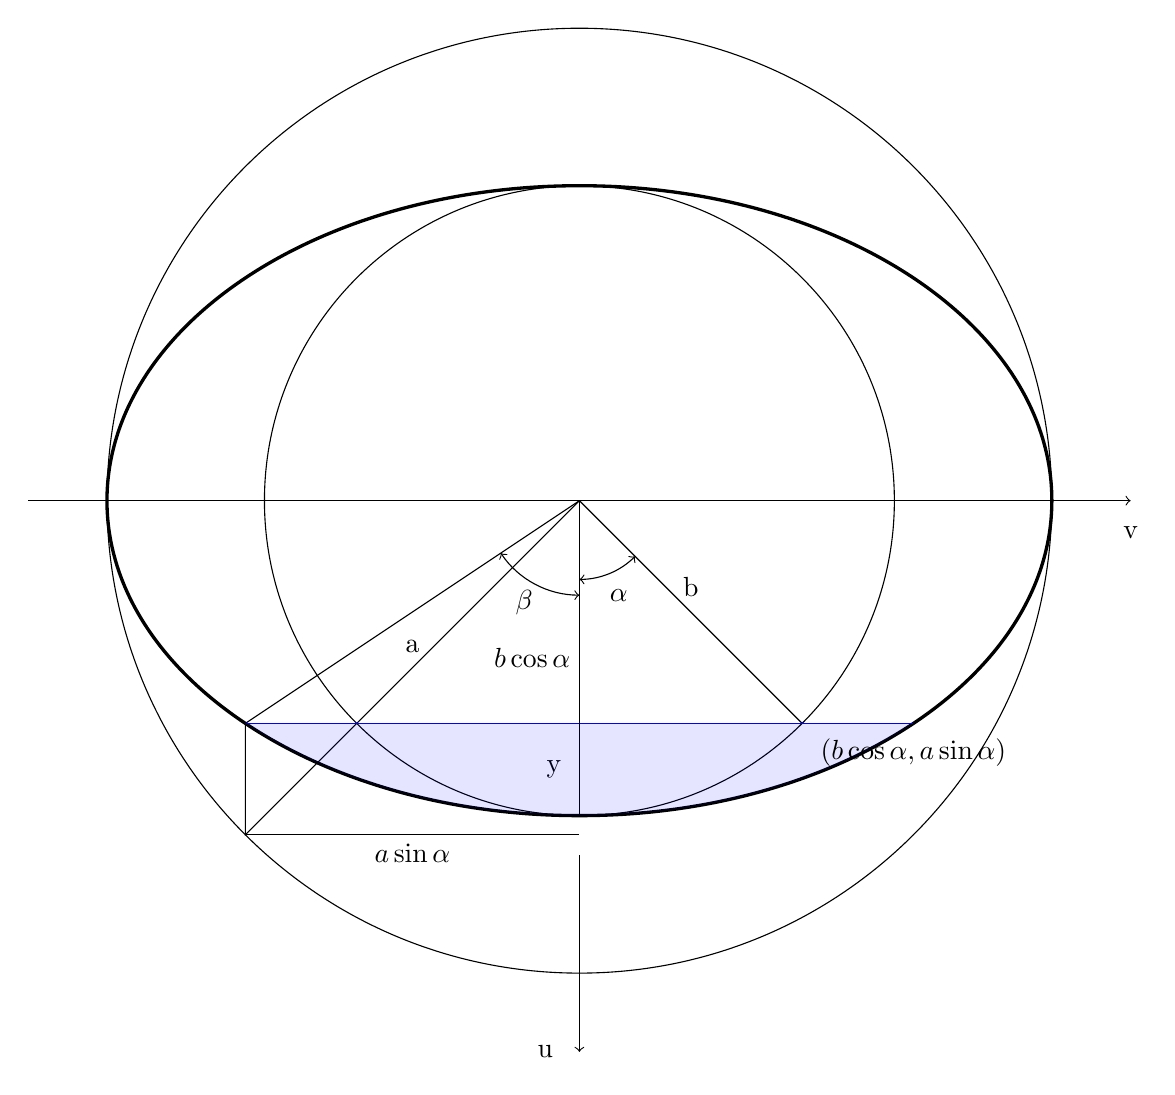
\begin{tikzpicture}

\draw (0,0) circle (6);
\draw (0,0) circle (4);
\draw [very thick](0,0) ellipse (6 and 4);

\draw[->](-7,0) --(7, 0) node[below =6]{v} ;
\draw[->](0, -4.5) --(0,-7) node[left =6]{u} ;


\draw (0,0)--node[above=2]{b} (2.828, -2.828);
\draw (0,0)--node[above=2]{a}(-4.242, -4.242)--(-4.242, -2.828);
\draw[blue] (-4.242, -2.828) -- (4.242, -2.828);
\draw (0,0)-- (0,-2.828)--node[left=3]{y} (0,-4);
\node at (-0.6, -2){$b\cos\alpha$};

\draw (-4.242, -4.242)--node[below]{$a\sin\alpha$}(0, -4.242);

\filldraw[fill=blue, opacity=0.1](-4.242, -2.828) arc[x radius=6, y radius = 4, start angle = 225, end angle=315];

\draw [<->] (0, -1) arc [radius=1, start angle=270, end angle=315];
\node at (0.5, -1.2) {$\alpha$};

\draw (0, 0) --(-4.242, -2.828);
\draw [<->] (0, -1.2) arc [radius=1.2, start angle=270, end angle=213.7];
\node at (-0.7, -1.3) {$\beta$};

\node at (4.242, -3.2) {$(b\cos\alpha, a\sin\alpha)$};

\end{tikzpicture}
\caption{Elliptical Section ($a \ge b$)}
\label{Fig:EllipseA}
\end{figure}

\begin{figure}[h]
\centering
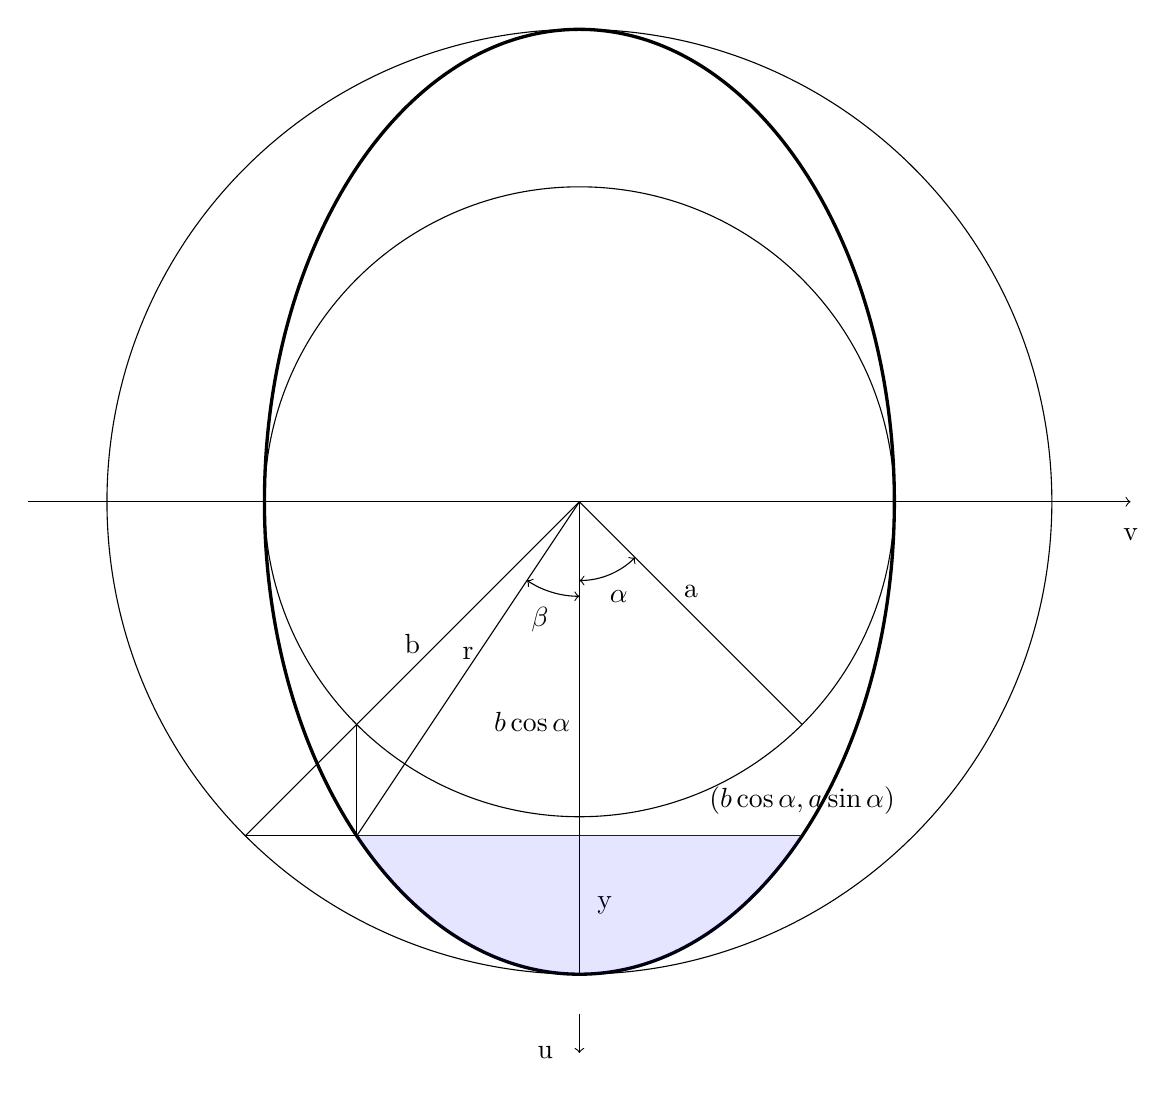
\begin{tikzpicture}
\draw (0,0) circle (6);
\draw (0,0) circle (4);
\draw [very thick](0,0) ellipse (4 and 6);
\draw[->](-7,0) --(7, 0) node[below =6]{v} ;
\draw[->](0, -6.5) --(0,-7) node[left =6]{u} ;

\draw (0,0)--node[above=2]{a} (2.828, -2.828);
\draw (0,0)--node[above=2]{b}(-4.242, -4.242);
\draw (-4.242, -4.242)--(-2.828, -4.242) -- (-2.828, -2.828);
\draw[blue] (-2.828, -4.242) --(2.828, -4.242);
\draw (0,-4.242)--node[right=3]{y} (0,-6);

\filldraw[fill=blue, opacity=0.1](-2.828, -4.242) arc[x radius=4, y radius = 6, start angle = 225, end angle=315];

\draw(0, 0) -- (0, -4.242);
\node at (-0.6, -2.8) {$b\cos\alpha$};

\draw [<->] (0, -1) arc [radius=1, start angle=270, end angle=315];
\node at (0.5, -1.2) {$\alpha$};

\draw [<->] (0, -1.2) arc [radius=1.2, start angle=270, end angle=236.31];
\node at (-0.5, -1.5) {$\beta$};


\draw (0, 0) --node[above]{r}(-2.828, -4.242);

\node at (2.828, -3.8) {$(b\cos\alpha, a\sin\alpha)$};

\end{tikzpicture}
\caption{Elliptical Section ($a < b$)}
\label{Fig:EllipseB}
\end{figure}

\begin{equation}
\begin{aligned}
u &= b\cos \alpha  \\
v &= a\sin \alpha  \\
\end{aligned}
\end{equation}

\begin{equation}
\tan\beta = \frac{a}{b}\tan\alpha
\end{equation}

\begin{equation}
\sin^2\alpha = \frac{\tan^2\alpha}{1+\tan^2\alpha}=\frac{b^2\tan^2\beta}{a^2+b^2\tan^2\beta} 
\end{equation}

\begin{equation}
\cos^2\alpha = \frac{1}{1+\tan^2\alpha}=\frac{a^2}{a^2+b^2\tan^2\beta}
\end{equation}

\begin{equation}
r^2 = a^2\sin^2\alpha + b^2\cos^2\alpha
\end{equation}

\begin{equation}
y = b(1 - \cos\alpha) 
\end{equation}

\begin{equation}
\cos\alpha =1 - \frac{y}{b}
\end{equation}

\begin{equation}
y' = \frac{\partial y}{\partial \alpha} = b \sin\alpha
\end{equation}

\subsection{Flow Area}
The flow area is
\begin{equation}
A = 2 \int_{b\cos\alpha }^b v du = -2ab\int^0_\alpha \sin^2tdt =  ab\int_0^\alpha (1 - \cos 2t) dt = ab(\alpha - \frac{1}{2}\sin 2 \alpha)
\end{equation}

\begin{equation}
A' = ab(1 - \cos2\alpha)
\end{equation}

\begin{equation}
A'' = 2ab\sin2\alpha
\end{equation}

\begin{equation}
\frac{\partial A}{\partial y} = \frac{A'}{y'} = 2a\sin\alpha = T_w
\end{equation}

\begin{equation}
\frac{\partial }{\partial \alpha}\left(\frac{\partial A}{\partial y}\right) = 2a\cos\alpha
\end{equation}

\begin{equation}
D_h = \frac{A'}{\frac{\partial A}{\partial y}} = \frac{b(\alpha - \frac{1}{2}\sin 2 \alpha)}{ 2\sin\alpha}
\end{equation}


\subsection{Wet Perimeter}
\subsubsection{$a \ge b$}
In the case of $a \ge b$ (Figure \ref{Fig:EllipseA}), the wet perimeter is
\begin{equation}
P =  2\int _0 ^{\alpha } \sqrt{a^2\cos^2t + b^2\sin^2t} dt =2 a\int _0 ^{\alpha } \sqrt{1 - \left(1 - b^2/a^2\right) \sin^2t} dt =  2aE(\alpha, \eta)
\end{equation}
with $\eta^2 = 1 - b^2/a^2$,  $E(\alpha, \zeta)$ as the Legendre ellitipcal integral of the second kind.

\begin{equation}
E(\alpha, \eta) = \alpha -\frac{1}{2}\eta^2\int_0^\alpha \sin^2 tdt - \frac{1}{2 \cdot 4}\eta^4\int_0^\alpha \sin^4 tdt - \frac{1 \cdot 3}{2 \cdot 4 \cdot 6}\eta^6\int_0^\alpha \sin^6 tdt + ...
\end{equation}

\begin{equation}
\begin{aligned}
\int \sin^n t dt &= -\frac{1}{n} \sin^{n-1} \cos t + \frac{n-1}{n} \int \sin^{n-2} t dt \\
\int_0^\alpha \sin^2 tdt &=  -\frac{1}{2}\sin \alpha \cos\alpha + \frac{1}{2}\alpha \\
\int_0^\alpha \sin^4 t dt &= -\frac{1}{4}\sin^3 \alpha  \cos \alpha + \frac{3}{4} \int_0^\alpha \sin^2 t dt \\
\int_0^\alpha \sin^6 t dt &= -\frac{1}{6}\sin^5 \alpha  \cos \alpha + \frac{5}{6} \int_0^\alpha \sin^4 t dt \\
\int_0^\alpha \sin^{2n} t dt &= -\frac{1}{2n}\sin^{2n-1} \alpha  \cos \alpha + \frac{2n-1}{2n} \int_0^\alpha \sin^{2n-2} t dt 
\end{aligned}
\end{equation}

\begin{center}
\begin{tabular}{| c | c | c | c | c | c | c | }
\hline
n & $a_n$ & $b_n$ & $c_n$ & $d_n$ & $e_n$ & $f_n$\\ 
\hline
1 & $-\frac{1}{2}\eta^2$              &  $-\frac{1}{2}$    & $\sin\alpha \cos\alpha$ &  $\frac{1}{2}$        & $b_1c_1 + d_1\alpha$   & $a_1e_1$ \\ 
2 & $a_1 \frac{\eta^2}{4}$          &  $-\frac{1}{4}$    &  $c_1 \sin^2\alpha$       &  $\frac{3}{4}$        & $b_2c_2 + d_2e_1$       & $a_2e_2$   \\  
3 & $a_2 \frac{\eta^2}{6}$          &  $-\frac{1}{6}$    &  $c_2 \sin^2\alpha$       &  $\frac{5}{6}$        & $b_3c_3 + d_3e_2$       & $a_3e_3$   \\  
n & $a_{n-1} \frac{\eta^2}{2n}$ &   $-\frac{1}{2n}$ &  $c_{n-1} \sin^2\alpha$ & $\frac{2n-1}{2n}$ & $b_nc_n + d_ne_{n-1}$ & $a_ne_n$  \\
\hline
\end{tabular}
\end{center}



\subsubsection{$a < b$}

For $a < b$, the wet perimeter is (Figure \ref{Fig:EllipseB})
\begin{equation}
P =  2\int _0 ^{\alpha } \sqrt{a^2\cos^2t + b^2\sin^2t} dt = 2b\int _0 ^{\alpha } \sqrt{1 - \left(1 - a^2/b^2\right) \cos^2t} dt =  2bF(\alpha, \zeta)
\end{equation}
with $\zeta^2 = 1 - a^2/b^2$.

\begin{equation}
F(\alpha, \eta) = \alpha - \frac{1}{2}\zeta^2\int_0^{\alpha} \cos ^2 t dt - \frac{1}{2^2 \cdot 2!}\zeta^4\int_0^{\alpha} \cos ^4 t dt - \frac{1 \cdot 3}{2^3 \cdot 3!}\zeta^6\int_0^{\alpha} \cos ^6 t dt - \cdot \cdot \cdot
\end{equation}

\begin{equation}
\begin{aligned}
\int \cos^n t dt &= \frac{1}{n} \sin t  \cos^{n-1} t + \frac{n}{n-1} \int \cos^{n-2} t dt \\
\int_0^\alpha \cos^2 t dt &= \frac{1}{2}\sin \alpha  \cos \alpha + \frac{1}{2} \alpha  \\
\int_0^\alpha \cos^4 t dt &= \frac{1}{4}\sin \alpha  \cos^3 \alpha + \frac{3}{4} \int_0^\alpha \cos^2 t dt \\
\int_0^\alpha \cos^6 t dt &= \frac{1}{6}\sin \alpha  \cos^5 \alpha + \frac{5}{6} \int_0^\alpha \cos^4 t dt \\
\int_0^\alpha \cos^{2n} t dt &= \frac{1}{2n}\sin \alpha  \cos^{2n-1} \alpha + \frac{2n-1}{2n} \int_0^\alpha \cos^{2n-2} t dt 
\end{aligned}
\end{equation}

For both cases,

\begin{equation}
P' = 2\sqrt{a^2\cos^2\alpha + b^2\sin^2\alpha} 
\end{equation}

\begin{equation}
P'' =-\frac{(a^2-b^2)\sin2\alpha}{\sqrt{a^2\sin^2\alpha + b^2\cos^2\alpha}} 
\end{equation}

\noindent Neton's method is used to calculate normal depth $y_n$,  critical depth $y_c$, $\alpha_{max}$, $y_{max}$, and $Q_{max}$.
%\begin{equation}
%\cos \alpha =1 - y/b 
%\end{equation}

%\begin{figure}[h]
%\centering
%\begin{tikzpicture}

%\draw (0,0) circle (3);
%\draw (0,0) circle (2);
%\draw [very thick](0,0) ellipse (3 and 2);


%\draw (0,0)--node[above=2]{b} (1.41421, -1.41421);
%\draw (0,0)--node[above=2]{a}(-2.12132, -2.12132)--(-2.12132, -1.41421);
%\draw[blue] (-2.12132, -1.41421) -- (2.12132, -1.41421);
%\draw (0,-1.41421)--node[right=3]{y} (0,-2);

%\filldraw[fill=blue, opacity=0.2](-2.12132, -1.41421) arc[x radius=3, y radius = 2, start angle = 225, end angle=315];

%\draw [<->] (-0.3536, -0.3536) arc [radius=0.5, start angle=225, end angle=315];
%\node at (-0.0, -0.8) {$\theta=2\alpha$};

%\node at (0.0, -3.5) {$(a) a > b$};

%\draw (7,0) circle (3);
%\draw (7,0) circle (2);
%\draw [very thick](7,0) ellipse (2 and 3);

%\draw (7,0)--node[above=2]{a} (8.41421, -1.41421);
%\draw (7,0)--node[above=2]{b}(4.87868, -2.12132)--(5.58579, -2.12132)--(5.58579,-1.41421);
%\draw[blue] (5.58579, -2.12132) --(8.41421, -2.12132);
%\draw (7,-2.12132)--node[right=3]{y} (7,-3);

%\filldraw[fill=blue, opacity=0.2](5.58579, -2.12132) arc[x radius=2, y radius = 3, start angle = 225, end angle=315];

%\draw [<->] (6.6465, -0.3536) arc [radius=0.5, start angle=225, end angle=315];
%\node at (7, -0.8) {$\theta=2\alpha$};

%\node at (7.0, -3.5) {$(b) a < b$};

%\end{tikzpicture}
%\end{figure}

%\subsection{Calculate Maximum Discharge Using Manning's Equation}
%\begin{equation}  
%Q = \frac{K_u}{n}AR^{2/3}S^{1/2} = \frac{K_u}{n}A^{5/3}P^{-2/3}S^{1/2},
%\end{equation}

%\begin{equation}  
%\frac{dQ}{d\theta} = \frac{K_u}{n} \left(\frac{5}{3}R^{2/3}\frac{\partial A}{\partial \theta} -  \frac{2}{3}R^{5/3}\frac{\partial P}{\partial \theta} \right) S^{1/2}=0,
%\end{equation}
%To reach maximum capacity, the $\alpha$ is solved using Newton-Raphson method

%\begin{equation}  
%\alpha _{i+1} = \alpha _i - \frac{f(\alpha _i)}{f'(\alpha_i)},
%\end{equation}

%with Eq. \ref{Eq:CircularMaxQ},

%\begin{equation}  
%f(\alpha) = 5A'P -  2AP' = 0,
%\end{equation}
%and
%\begin{equation}  
%f'(\alpha) = 3A'P' + 5A''P - 2AP''.
%\end{equation}

%\subsection{Calculate Normal Depth}
%For $Q$ less than $Q_{max}$,
%\begin{equation}  
%\alpha_{i+1} = \alpha_i -\frac{f_d(\alpha_{i})}{f'_d(\alpha_{i})}
%\end{equation}
%where
%\begin{equation}  
%f_d(\alpha_{i})= \frac{K_u}{n}A^{5/3}P^{-2/3}S^{1/2} - Q 
%\end{equation}

%\begin{equation}  
%f'_d(\alpha_{i})= \frac{K_u}{n}\left(\frac{5}{3}R^{2/3}A' -  \frac{2}{3}R^{5/3}P'\right)S^{1/2}
%\end{equation}



%\subsection{Calculate Critical Depth}

%\begin{equation}  
%\frac{\partial A}{\partial y} (\alpha)= \frac{\frac{\partial A}{\partial \alpha}}{\frac{\partial y}{\partial \alpha}}=\frac{ab(1 - \cos2\alpha)}{b\sin \alpha} = 2a\sin \alpha
%\end{equation}

%\begin{equation}  
%\frac{\partial}{\partial \alpha} \left(\frac{\partial A}{\partial y} \right) =2  a \cos \alpha
%\end{equation}


%\begin{equation}  
%f_c(\alpha)= gA^3 - Q^2\frac{\partial A}{\partial y} =  gA^3 - 2aQ^2 \sin\alpha
%\end{equation}

%\begin{equation}  
%f'_c(\alpha)= 3gA^2\frac{\partial A}{\partial \alpha} - Q^2\frac{\partial}{\partial \alpha} \left(\frac{\partial A}{\partial y} \right)
%\end{equation}


\section{Arc}

%\subsection{Geometry}
The geometry of an arc is determined by $r_b$, $r_t$, $r_c$, and $rise$. 
\begin{equation}
\begin{aligned}
r_b & = AB = BO = BE \\
r_t & = AC = CG \\
r_c & = DE = DF = DG \\
c & = BC =BO - CO = BO - (OG - CG) =  r_b + r_t - rise \\
\end{aligned}
\end{equation}

\begin{figure}[h]
\centering
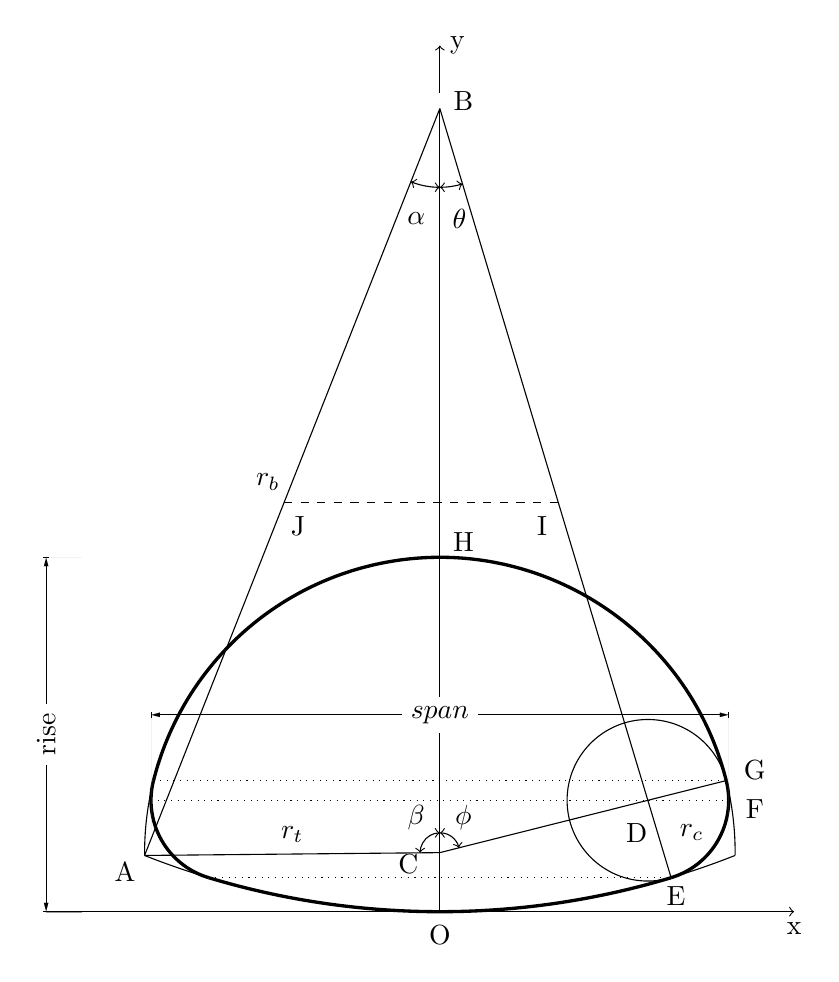
\begin{tikzpicture}

% base arc (thin) to A
\draw (-3.75, 0.714) arc[ x radius=10.2, y radius = 10.2, start angle = 248.43, end angle=291.57];
% BO
\draw (0,0) -- (0, 10.2);
% BA
\draw (0,10.2)--node[left=1]{$r_b$}(-3.75, 0.714);

\draw [<->] (0, 9.2) arc [radius=1, start angle=270, end angle=248.43];
\node at (-0.3, 8.8) {$\alpha$};

\draw [<->] (0, 9.2) arc [radius=1, start angle=270, end angle=286.74];
\node at (0.25, 8.8) {$\theta$};

% top arc (thin)
\draw (3.75, 0.714) arc[ x radius=3.75, y radius = 3.75, start angle = -0.55, end angle=180.55];
% CA
\draw (0,0.75)--node[above=0.5]{$r_t$}(-3.75, 0.714);

\draw [<->] (0, 1.0) arc [radius=0.25, start angle=90, end angle=180.55];
\node at (-0.3, 1.2) {$\beta$};

\draw [<->] (0, 1.0) arc [radius=0.25, start angle=90, end angle=14.12];
\node at (0.3, 1.2) {$\phi$};



\node at (3.2, 1.0) {$r_c$};
\node at (0, -0.3) {O};
\node at (-4.0, 0.5) {A};
\node at (0.3, 10.3) {B};
\node at (-0.4, 0.6) {C};
\node at (2.5, 1.0) {D};
\node at (3.0, 0.2) {E};
\node at (4.0, 1.3) {F};
\node at (4.0, 1.8) {G};
\node at (0.3, 4.7) {H};
\node at (1.3, 4.9) {I};
\node at (-1.8, 4.9) {J};

% IJ
\draw[dashed,thin] (-1.98,5.2) -- (1.5, 5.2);


\draw (2.642,1.415) circle [radius = 1.026];

\draw (0, 10.2) -- (2.937, 0.432);                    % BE
\draw [thin] (3.637, 1.665) -- (0,0.75);           % CG

\draw [very thick](-2.937, 0.432) arc[ x radius=10.2, y radius = 10.2, start angle = 253.26, end angle=286.74];
\draw [dotted, thin] (-2.937, 0.432) -- (2.937, 0.432);   % EE'

\draw [very thick]( 3.637, 1.665) arc[ x radius=3.75, y radius = 3.75, start angle = 14.121, end angle=165.88];
\draw[dotted, thin](-3.637, 1.665) -- (3.637, 1.665);      % GG'

\draw [very thick]( -3.637, 1.665) arc[ x radius=1.026, y radius = 1.026, start angle = 165.88, end angle=253.26];
\draw [very thick]( 3.637, 1.665) arc[ x radius=1.026, y radius = 1.026, start angle = 14.12, end angle=-73.26];
\draw[dotted, thin](-3.668, 1.415) -- (3.668, 1.415);    % FF'

\dimline [extension start length=0.2, extension end length=0.2]{(-3.668, 2.5)}{(3.668, 2.5)}{$span$}
\dimline [extension start length=0.1, extension end length=0.1]{(-5.0, 0)}{(-5.0, 4.5)}{rise}

\draw[->](-5, 0) --(4.5,0) node[below =0.5]{x} ;
\draw[->](0, 10.4) --(0,11) node[right =0.2]{y} ;

\end{tikzpicture}
\caption{Arc Section}
\label{Fig:Arc}
\end{figure}

\begin{equation}
\begin{aligned}
\cos\alpha &= \frac{r_b^2 + c^2 - r_t^2}{2r_b c} \\%= \frac{AB^2 + BC^2 - AC^2}{2 AB\times BC} \\
\cos\beta &= \frac{r_t^2 + c^2 - r_b^2}{2r_t c} \\ %= \frac{AC^2 + BC^2 - AB^2}{2 AC\times BC} \\
\cos\theta &= \frac{(r_b - r_c)^2 + c^2 - (r_t - r_c)^2}{2(r_b - r_c) c} \\ %= \frac{BD^2 + BC^2 - CD^2}{2 BD\times BC}\\
\cos\phi &= \frac{(r_t - r_c)^2 + c^2 - (r_b - r_c)^2}{2(r_t - r_c) c}  \\%= \frac{CD^2 + BC^2 - BD^2}{2 CD\times BC} \\
\end{aligned}
\end{equation}

\begin{equation}
\begin{aligned}
x_A & = r_b  \sin\alpha \\
y_A & = r_b  (1 - \cos\alpha) \\
y_B & = r_b \\
y_C & = rise - r_t = OG - CG \\
x_D &= (r_b -  r_c ) \sin\theta = (r_t - r_c) \sin \phi\\
y_D &= r_b - (r_b -  r_c ) \cos\theta = y_F \\
x_E & = r_b  \sin\theta \\
y_E & = r_b (1 - \cos\theta)\\
x_F & = x_D + r_c = span/2\\
x_G &= r_t \sin\phi \\
y_G &= y_C + r_t \cos\phi = rise - r_t (1 - \cos\phi) \\
y_H & = rise \\
\end{aligned}
\end{equation}

\begin{equation}
\begin{aligned}
A_E & =r_b^2(\theta - \sin \theta \cos \theta)  \\
P_E & =2  r_b \theta \\
T_E & = 2 r_b \sin \theta  \\
A_F & = A_E +   r_c^2 (\pi/2 - \theta) +  (x_E + x_D)(y_D-y_E)  \\
P_F & = P_E + 2  r_c (\pi/2 - \theta) \\
T_F & =  2 (x_D + r_c)  \\
A_G & = A_F +   r_c^2 (\pi/2 - \phi) +  (x_D + x_G)(y_G-y_D)   \\
P_G & = P_F + 2  r_c (\pi/2 - \phi) \\
T_G & =  2 r_t \sin \phi  \\
A_T & = A_G + r_t^2(\phi - \sin\phi\cos\phi) \\
P_T &= P_G + 2 r_t\phi
\end{aligned}
\end{equation}

\begin{figure}[h]
\centering
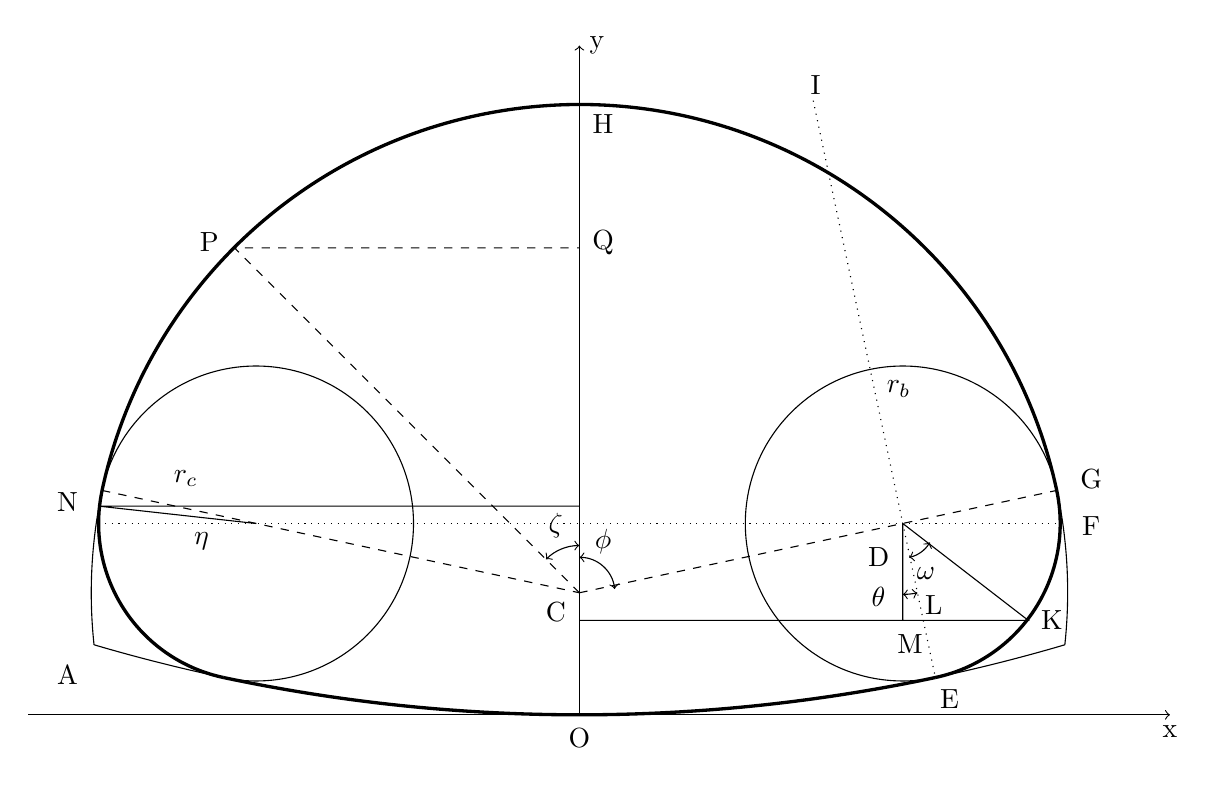
\begin{tikzpicture}

% base arc (thin) to A
\draw (-6.165, 0.890) arc[ x radius=21.8, y radius = 21.8, start angle = 253.57, end angle=286.43];
% BO
%\draw (0,0) -- (0, 21.8);

% BA
%\draw (0,21.8)--node[right=1]{$r_b$}(6.165, 0.89);

%\draw [dotted](-4.13,7.8)--node[left=1]{$r_b$}(-6.165, 0.89);  % JA

\draw [dotted](2.97,7.8)--node[right=1]{$r_b$}(4.521, 0.474);  % IE

%\draw [<->] (0, 20.8) arc [radius=1, start angle=270, end angle=286.43];
%\node at (0.2, 20.3) {$\alpha$};

%\draw [<->] (0, 20.8) arc [radius=1, start angle=270, end angle=258.03];
%\node at (-0.2, 20.3) {$\theta$};

% top arc (thin)
\draw (6.165, 0.890) arc[ x radius=6.2, y radius = 6.2, start angle = -6.11, end angle=186.11];

%\draw [dashed](0,1.55)--node[above=0.5]{$r_t$}(-6.165, 0.89); % CA

%\draw [dashed](0,1.55)--(4.521, 0.474);  % CE

\draw [dashed](0,1.55)--( 6.062, 2.850);  % CG

\draw [<->] (0, 2.0) arc [radius=0.45, start angle=90, end angle=6.11];
\node at (0.3, 2.2) {$\phi$};

%\draw [<->] (0, 2.0) arc [radius=0.45, start angle=90, end angle=192.1];
%\node at (-0.5, 2.2) {$\beta$};

\node at (-5.0, 3.0) {$r_c$};

\node at (0, -0.3) {O};
\node at (-6.5, 0.5) {A};
%\node at (0.3, 22.0) {B};
\node at (-0.3, 1.3) {C};
\node at (3.8, 2.0) {D};
\node at (4.7, 0.2) {E};
\node at (6.5, 2.4) {F};
\node at (6.5, 3.0) {G};
\node at (0.3, 7.5) {H};

\node at (3, 8) {I};
%\node at (-4, 08) {J};
\node at (6.0, 1.2) {K};
\node at (4.5, 1.4) {L};
\node at (4.2, 0.9) {M};
%\node at (0.3, 0.9) {K};
%\node at (0.3, 0.4) {L};
%\node at (6.8, 2.7) {N};

% circucle left
\draw (-4.107,2.43) circle [radius = 2.0];

%BF
%\draw (0, 21.8) -- (-4.521, 0.474);

%CG' 
\draw  [dashed](-6.062, 2.850) -- (0,1.55);

%bottom
\draw [very thick](-4.521, 0.474) arc[ x radius=21.8, y radius = 21.8, start angle = 258.03, end angle=281.97];
%top
\draw [very thick]( 6.062, 2.850) arc[ x radius=6.2, y radius = 6.2, start angle = 12.1, end angle=167.9];
%left
\draw [very thick]( -4.521, 0.474) arc[ x radius=2.0, y radius = 2.0, start angle = 258.03, end angle=167.9];
%right
\draw [very thick](  4.521, 0.474) arc[ x radius=2.0, y radius = 2.0, start angle = -78.03, end angle=12.1];

%\dimline [extension start length=0.1, extension end length=0.1]{(-7.0, 0)}{(-7.0, 7.75)}{rise}

\draw[->](-7, 0) --(7.5,0) node[below =0.5]{x} ;
\draw[->](0, 0) --(0,8.5) node[right =0.2]{y} ;

\draw(0, 1.2)--(5.7, 1.2)--(4.107,2.43) --(4.107, 1.2) ;

\draw [<->] (4.107, 1.53) arc [radius=0.9, start angle=270, end angle=281.97];
\node at (3.8, 1.5) {$\theta$};

\draw [<->] (4.187, 2.0) arc [radius=0.4, start angle=281.97, end angle=330];
\node at (4.4, 1.8) {$\omega$};

%\draw (-4.521, 0.474) --(0, 0.474);

%\draw(0, 1.2)--(-5.7, 1.2)--(-4.107,2.43) --(-4.107, 1.2) ;
%\draw [<->] (-4.107, 2.0) arc [radius=0.4, start angle=270, end angle=210];
%\node at (-4.4, 1.8) {$\omega$};
\node at (-4.8, 2.2) {$\eta$};

% circucle right
\draw (4.107,2.43) circle [radius = 2.0];

\draw[dotted](-6.107, 2.43)--(6.107, 2.43);

\draw(0, 2.65)--(-6.1, 2.65)--(-4.107,2.43);
\node at (-6.5, 2.7) {N};


\draw [dashed](0,1.55)--(-4.38, 5.93)--(0, 5.93);    % CP

\node at (-4.7, 6) {P};
\node at (0.3, 6) {Q};

\draw [<->] (0, 2.15) arc [radius=0.6, start angle=90, end angle=135];
\node at (-0.3, 2.4) {$\zeta$};


\end{tikzpicture}
\caption{Arc Section}
\label{Fig:Arc1}
\end{figure}

\noindent For $0 \le y \le y_E$, $0 \le t \le \theta$
\begin{equation}
\begin{aligned}
x & = r_b \sin t \\
y & = r_b (1 - \cos t) \\
y' & = r_b \sin t = \frac{\partial y}{\partial t}\\
A & = r_b^2(t - \sin t \cos t) \\
A' & = r_b^2(1 - \cos 2t)  = \frac{\partial A}{\partial t}\\
\frac{\partial A}{\partial y} &= 2 r_b\sin t = T_w\\
\frac{\partial}{\partial t}\left( \frac{\partial A}{\partial y}\right) &= 2 r_b\cos t \\
P & =2  r_b t\\
%T & = 2 r_b \sin t \\
\end{aligned}
\end{equation}

\noindent For $y_E \le y \le y_F$, $0 \le w \le \pi/2 - \theta $
\begin{equation}
\begin{aligned}
x &= x_D +  r_c \sin(\omega +\theta) \\
x_L &= x_D +  r_c \cos(\omega +\theta) \tan\theta \\
x'_L &= -  r_c \sin(\omega +\theta) \tan\theta \\
x''_L &=-  r_c \cos(\omega +\theta) \tan\theta \\
y &= y_D - r_c \cos(\omega +\theta) \\
y' &=  r_c \sin(\omega +\theta) \\
y'' &=  r_c \cos(\omega +\theta) \\
A &= A_E +  r_c^2 \omega - r_c^2 \sin(\omega + \theta) \cos(\omega + \theta) + r_c^2 \cos^2(\omega + \theta) \tan\theta  + (x_E +x_L) (y - y_E)  \\
A' &=  r_c^2 - r_c^2 \cos 2(\omega + \theta) - r_c^2 \sin 2(\omega + \theta) \tan\theta  + (x_E +x_L)  y' +  x'_L (y - y_E) \\
   &=  2 r_c^2 \sin^2(\omega + \theta) - 2 r_c^2 \sin(\omega + \theta) \cos(\omega + \theta)\tan\theta  + (x_E +x_L)  y' +  x'_L (y - y_E) \\
%A'' &=  2 r_c^2 \sin \left[2(\omega + \theta)\right] - 2 r_c^2 \cos [2(\omega + \theta)] \tan\theta  + (x_E +x_L)  y'' + x_L'y' +  x''_L (y - y_E) + x'_Ly'\\
\frac{\partial A}{\partial y} &= \frac{A'}{y'} = \frac{ 2 r_c^2 \sin ^2(\omega + \theta) -2 r_c^2 \sin (\omega + \theta) \cos (\omega + \theta) \tan\theta}{r_c \sin(\omega +\theta)} + x_E + x_L  - (y - y_E) \tan \theta\\
  &= 2r_c\sin(\omega + \theta) - 2r_c\cos(\omega + \theta)\tan\theta + x_E + x_D +  r_c \cos(\omega +\theta) \tan\theta \\
  & -  \left[y_D - r_c \cos(\omega +\theta) - y_E\right] \tan \theta \\
  &= 2r_c\sin(\omega + \theta) + x_E + x_D - (y_D - y_E) \tan\theta = 2x_D + 2r_c\sin(\omega + \theta) = T_w\\
\frac{\partial}{\partial \omega}\left( \frac{\partial A}{\partial y}\right) &=  2r_c\cos(\omega + \theta) \\
P &= P_E + 2 r_c \omega \\
%T &= 2 x_D + 2 r_c \sin(\omega + \theta) \\
\end{aligned}
\end{equation}

%\begin{equation}
%\begin{aligned}
%A' & =  r_c^2 - r_c^2 \cos 2(\omega + \theta) - r_c^2 \sin 2(\omega + \theta)\tan\theta + x_E y' + x_L'y + x_Ly' - x_L'y_E  \\
%A' & =  r_c^2 [1 - \cos 2(\omega + \theta) - \sin 2(\omega + \theta)\tan\theta] +  r_c(x_E + x_L) \sin (\omega + \theta) -  r_c (y - y_E) \sin(\omega + \theta)\tan\theta \\
%\end{aligned}
%\end{equation}


%where

%\begin{equation}
%\begin{aligned}
%x_K & = x_D + r_c\sin (\omega + \theta) \\ 
%y_K & = y_E + r_c [\cos\theta - \cos(\omega + \theta)] \\
%x_L  & = x_D +  (y_D - y)\tan\theta \\
%\end{aligned}
%\end{equation}


%$A_{HJF} =A_{DHF} - A_{DHI} = \frac{1}{2}r_c^2 (\omega - \theta) - \frac{1}{2}r_c^2 (\sin\omega - \sin\theta)\cos\omega$

%$FL = r_b \sin\theta$

%$KL = y_H - y_F = y - r_b (1 - \cos\theta) $

%$KI = FL - KL \tan \theta = r_b \sin\theta - [y - r_b (1 - \cos\theta)] \tan\theta$

%$A_{IKLF} =\frac{1}{2} (x_F +x_I) (y - y_F)$

%$A_H = A_F + 2A_{HJF} + 2 A_{IKLF} = A_F + r_c^2 (\omega - \theta) - r_c^2 (\sin\omega - \sin\theta)\cos\omega + (x_F +x_I) (y - y_F) $



%For $y = y_M$, $w = \frac{\pi}{2}$
%\begin{equation}
%\begin{aligned}
%A_M & = A_F + r_c^2(\frac{\pi}{2} - \theta) + (x_D + x_F)(y_D - y_F) \\
%P_M & = P_F + 2 r_c (\frac{\pi}{2} - \theta) \\
%T_M & = 2(r_b -  r_c ) \sin\theta + 2 r_c \\
%\end{aligned}
%\end{equation}

\noindent For $y_F \le y \le y_G$, $0 \le \eta \le  \pi/2-\phi$
\begin{equation}
\begin{aligned}
x & = x_D + r_c \cos\eta \\
y & = y_D + r_c \sin \eta \\
A & = A_F + r_c^2 \eta + (2x_D + r_c\cos\eta)r_c\sin\eta  \\
P & = P_F + 2 r_c \eta \\
%T & = 2 x_D + 2 r_c \cos\eta \\
y' & = r_c \cos \eta \\
%y'' & = -r_c \sin \eta \\
A' & = r_c^2 + 2x_D r_c\cos\eta + r_c^2 \cos(2\eta)  \\
%A'' & = -2x_D r_c\sin\eta - 2 r_c^2 \sin(2\eta)  \\
\frac{\partial A}{\partial y} &= \frac{A'}{y'} = \frac{ r_c^2 + 2x_D r_c\cos\eta + r_c^2 \cos(2\eta)}{r_c \cos \eta} =  2x_D + 2r_c\cos\eta = T_w \\
\frac{\partial}{\partial \eta}\left( \frac{\partial A}{\partial y}\right) & = - 2 r_c \sin \eta \\
\end{aligned}
\end{equation}

\noindent For $y_G \le y \le y_H$, $0 \le \zeta \le \phi$
\begin{equation}
\begin{aligned}
y & = y_C + r_t \cos \zeta \\
A & = A_T - r_t^2(\zeta - \sin \zeta \cos \zeta) \\
P & = P_T - 2 r_t \zeta = P_G + 2 r_t (\phi - \zeta) \\
%T & = 2r_t \sin \zeta \\
y' & = -r_t \sin \zeta \\
%y'' & = -r_t \cos \zeta \\
A' &= - r_t^2[1 - \cos(2\zeta)] \\
A'' &= -2  r_t^2 \sin(2\zeta) \\
P'(\zeta) & = -2 r_t \\
P''(\zeta) & = 0 \\
\frac{\partial A}{\partial y} &= \frac{A'}{y'} = 2 r_t \sin \zeta = T_w\\
\frac{\partial}{\partial t}\left( \frac{\partial A}{\partial y}\right) &=  2 r_t \cos \zeta\\
\end{aligned}
\end{equation}


%\begin{figure}[h]
%\centering
%\begin{tikzpicture}

% base arc (thin) to A
%\draw (-6.165, 0.890) arc[ x radius=21.8, y radius = 21.8, start angle = 253.57, end angle=286.43];
% BO
%\draw (0,0) -- (0, 21.8);
% BA
%\draw (0,21.8)--node[right=1]{$r_b$}(6.165, 0.89);

%\draw [<->] (0, 20.8) arc [radius=1, start angle=270, end angle=286.43];
%\node at (0.2, 20.3) {$\alpha$};

%\draw [<->] (0, 20.8) arc [radius=1, start angle=270, end angle=258.03];
%\node at (-0.2, 20.3) {$\theta$};

% top arc (thin)
%\draw (6.165, 0.890) arc[ x radius=6.2, y radius = 6.2, start angle = -6.11, end angle=186.11];
% CA
%\draw (0,1.55)--node[above=0.5]{$r_t$}(6.165, 0.89);

%\draw [<->] (0, 2.0) arc [radius=0.45, start angle=90, end angle=-6.11];
%\node at (0.5, 2.2) {$\beta$};

%\draw [<->] (0, 2.0) arc [radius=0.45, start angle=90, end angle=167.9];
%\node at (-0.3, 2.2) {$\phi$};

%\node at (-5.0, 3.0) {$r_c$};
%\node at (0, -0.3) {O};
%\node at (6.5, 0.5) {A};
%\node at (0.3, 22.0) {B};
%\node at (-0.5, 1.4) {C};
%\node at (0.3, 7.5) {G};
%\node at (-3.8, 2.0) {D};
%\node at (-4.7, 0.2) {E};
%\node at (-6.5, 3.0) {F};
%\node at (-6.0, 1.2) {H};
%\node at (-4.5, 1.4) {I};
%\node at (-4.2, 0.9) {J};
%\node at (0.3, 0.9) {K};
%\node at (0.3, 0.4) {L};
%\node at (-6.8, 2.7) {N};
%\node at (-6.5, 2.4) {M};
% circucle left
%\draw (-4.107,2.43) circle [radius = 2.0];

%BF
%\draw (0, 21.8) -- (-4.521, 0.474);

%CE 
%\draw  (-6.062, 2.850) -- (0,1.55);

%bottom
%\draw [very thick](-4.521, 0.474) arc[ x radius=21.8, y radius = 21.8, start angle = 258.03, end angle=281.97];
%top
%\draw [very thick]( 6.062, 2.850) arc[ x radius=6.2, y radius = 6.2, start angle = 12.1, end angle=167.9];
%left
%\draw [very thick]( -4.521, 0.474) arc[ x radius=2.0, y radius = 2.0, start angle = 258.03, end angle=167.9];
%right
%\draw [very thick](  4.521, 0.474) arc[ x radius=2.0, y radius = 2.0, start angle = -78.03, end angle=12.1];

%\dimline [extension start length=0.1, extension end length=0.1]{(-7.0, 0)}{(-7.0, 7.75)}{rise}

%\draw[->](-7, 0) --(7.5,0) node[below =0.5]{x} ;
%\draw[->](0, 22.0) --(0,22.5) node[right =0.2]{y} ;

%\draw(0, 1.2)--(-5.7, 1.2)--(-4.107,2.43) --(-4.107, 1.2) ;
%\draw [<->] (-4.107, 2.0) arc [radius=0.4, start angle=270, end angle=210];
%\node at (-4.4, 1.8) {$\omega$};

%\draw (-4.521, 0.474) --(0, 0.474);

%\draw(0, 1.2)--(-5.7, 1.2)--(-4.107,2.43) --(-4.107, 1.2) ;
%\draw [<->] (-4.107, 2.0) arc [radius=0.4, start angle=270, end angle=210];
%\node at (-4.4, 1.8) {$\omega$};

% circucle right
%\draw (4.107,2.43) circle [radius = 2.0];

%\draw(-6.107, 2.43)--(6.107, 2.43);

%\draw(0, 2.65)--(-6.1, 2.65)--(-4.107,2.43);

%\end{tikzpicture}
%\caption{Arc Section}
%\label{Fig:Arc1}
%\end{figure}

%\subsection{Calculate Maximum Discharge Using Manning's Equation}
\noindent Maximum discharge occurs close to the top of arch, the $\zeta_{max}$ is solved using Newton's method

\begin{equation}  
\zeta _{i+1} = \zeta _i - \frac{f(\zeta _i)}{f'(\zeta_i)},
\end{equation}

\noindent with %Eq. \ref{Eq:MaxQ},

\begin{equation}  
f(\zeta) = 5A'P -  2AP',
\end{equation}
and
\begin{equation}  
f'(\zeta) = 3A'P' + 5A''P - 2AP''.
\end{equation}

%\subsection{Calculate Normal Depth}
%For $Q$ less than $Q_{max}$,
%\begin{equation}  
%\alpha_{i+1} = \alpha_i -\frac{f_d(\alpha_{i})}{f'_d(\alpha_{i})}
%\end{equation}
%where
%\begin{equation}  
%f_d(\alpha_{i})= \frac{K_u}{n}A^{5/3}P^{-2/3}S^{1/2} - Q 
%\end{equation}

%\begin{equation}  
%f'_d(\alpha_{i})= \frac{K_u}{n}\left(\frac{5}{3}R^{2/3}A' -  \frac{2}{3}R^{5/3}P'\right)S^{1/2}
%\end{equation}

%\subsection{Critical Flow}
%Critical flow occurs when the specific energy of the cross-section
%\begin{equation}
%E = \frac{v^2}{2g} + y =\frac{Q^2}{2gA^2} + y 
%\end{equation}
%reaches a minimum. Namely,
%\begin{equation}
%\frac{\partial E}{\partial y} =  -\frac{Q^2}{gA^3}\frac{\partial A}{\partial y} + 1 = 0
%\end{equation}
%Newton-Raphson method is used to calculate critical depth as
%\begin{equation}  
%y_{c,i+1} = y_{c,i} -\frac{f(y_{c,i})}{f'(y_{c,i})}
%\end{equation}
%where
%\begin{equation}  
%f_c(y)= gA^3 - Q^2\frac{\partial A}{\partial y} 
%\end{equation}

%\begin{equation}  
%f'_c(y)= 3gA^2\frac{\partial A}{\partial y} - Q^2\frac{\partial ^2A}{\partial y^2} 
%\end{equation}

%\begin{equation}  
%f_c(y_{i})= 1 - \frac{Q^2}{gA^3}\frac{\partial A}{\partial y} 
%\end{equation}

%\begin{equation}  
%f'_c(y_{i})= \frac{Q^2}{gA^3} \left[ 3 \left(\frac{\partial A}{\partial y}\right)^2 - A\frac{\partial ^2 A}{\partial y^2}   \right] 
%\end{equation}

%for A and y are parameterized as a function of $t$ with $A=A(t)$, $A'=\frac{\partial A(t)} {\partial t}$, $y=y(t)$, $y'=\frac{\partial y(t)}{\partial t}$, 

%\begin{equation}  
%t_{c,i+1} = t_{c,i} -\frac{f(t_{c,i})}{f'(t_{c,i})}
%\end{equation}

%\begin{equation}  
%f_c(t)= gA^3(t) - Q^2\frac{\partial A}{\partial y}(t) 
%\end{equation}

%\begin{equation}  
%f'_c(t)= 3gA^2\frac{\partial A}{\partial t} - Q^2\frac{\partial}{\partial t}\left(\frac{\partial A}{\partial y}\right) 
%\end{equation}

%\begin{equation}  
%f_c(t)= 1 - \frac{Q^2}{gA^3}\frac{A'}{y'} 
%\end{equation}

%\begin{equation}  
%f'_c(t)= \frac{Q^2}{gA^3} \left[ 3 \left(\frac{\partial A}{\partial y}\right)^2 - A\frac{\partial ^2 A}{\partial y^2}   \right] 
%\end{equation}





\bibliographystyle{plain}
\bibliography{OpenChannel}

\end{document}
